%\newpage
\section{SORA Payload Description}
\label{sec:Hardware}

%\begin{figure}[t!]
%\begin{center}
%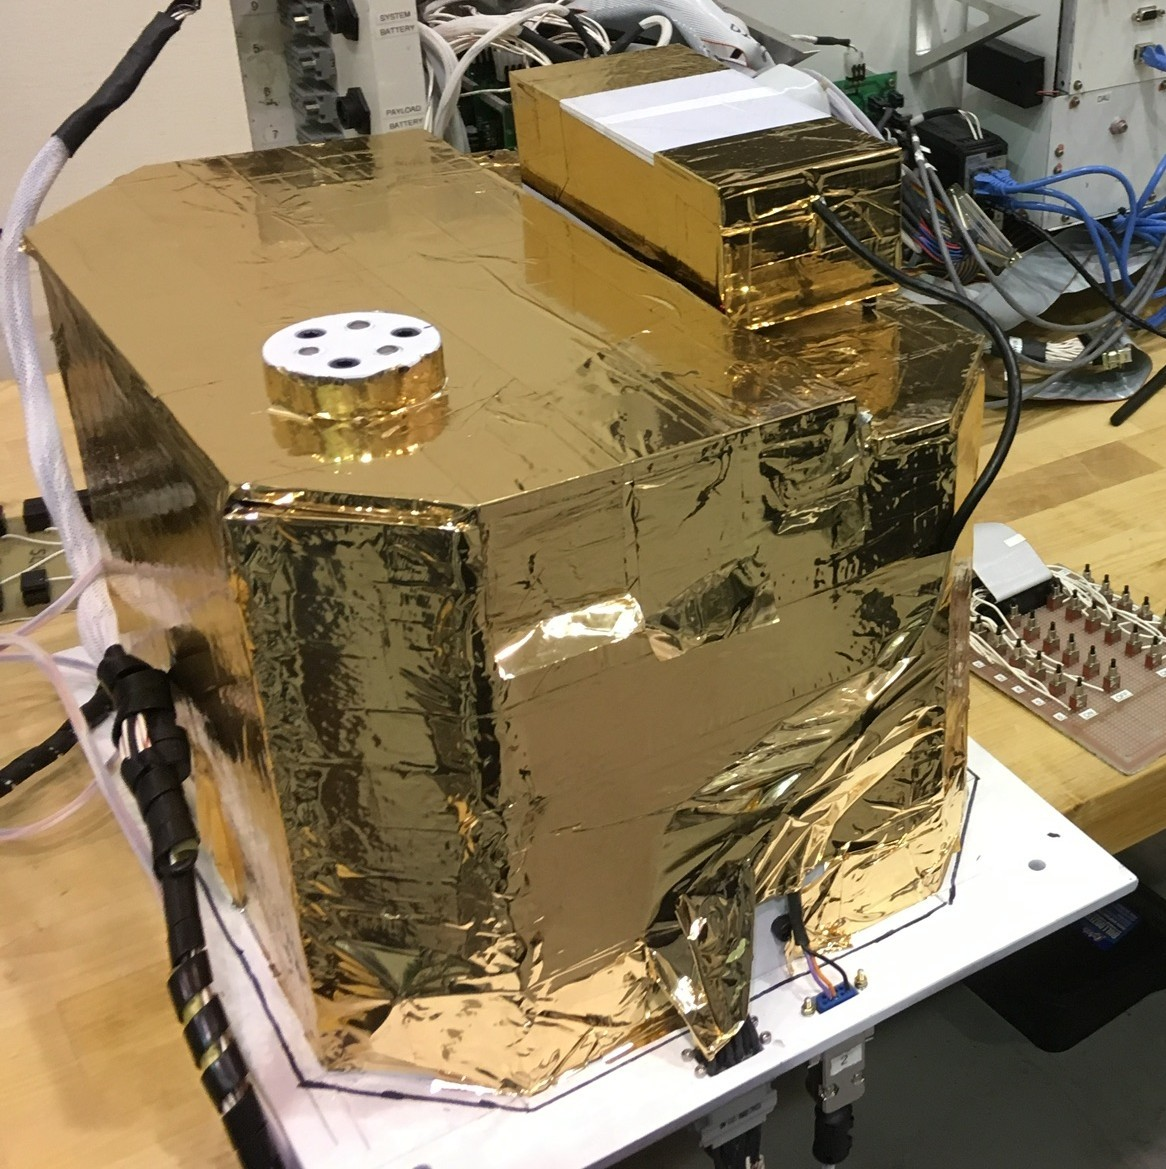
\includegraphics[width=0.60\textwidth]{./Figures/sora.JPG}
%\caption{SORA payload.}
%\label{fig:payload} 
%\end{center}
%\end{figure}

\begin{figure}[t]
  \begin{center}
    \begin{minipage}[c]{0.45\linewidth}
      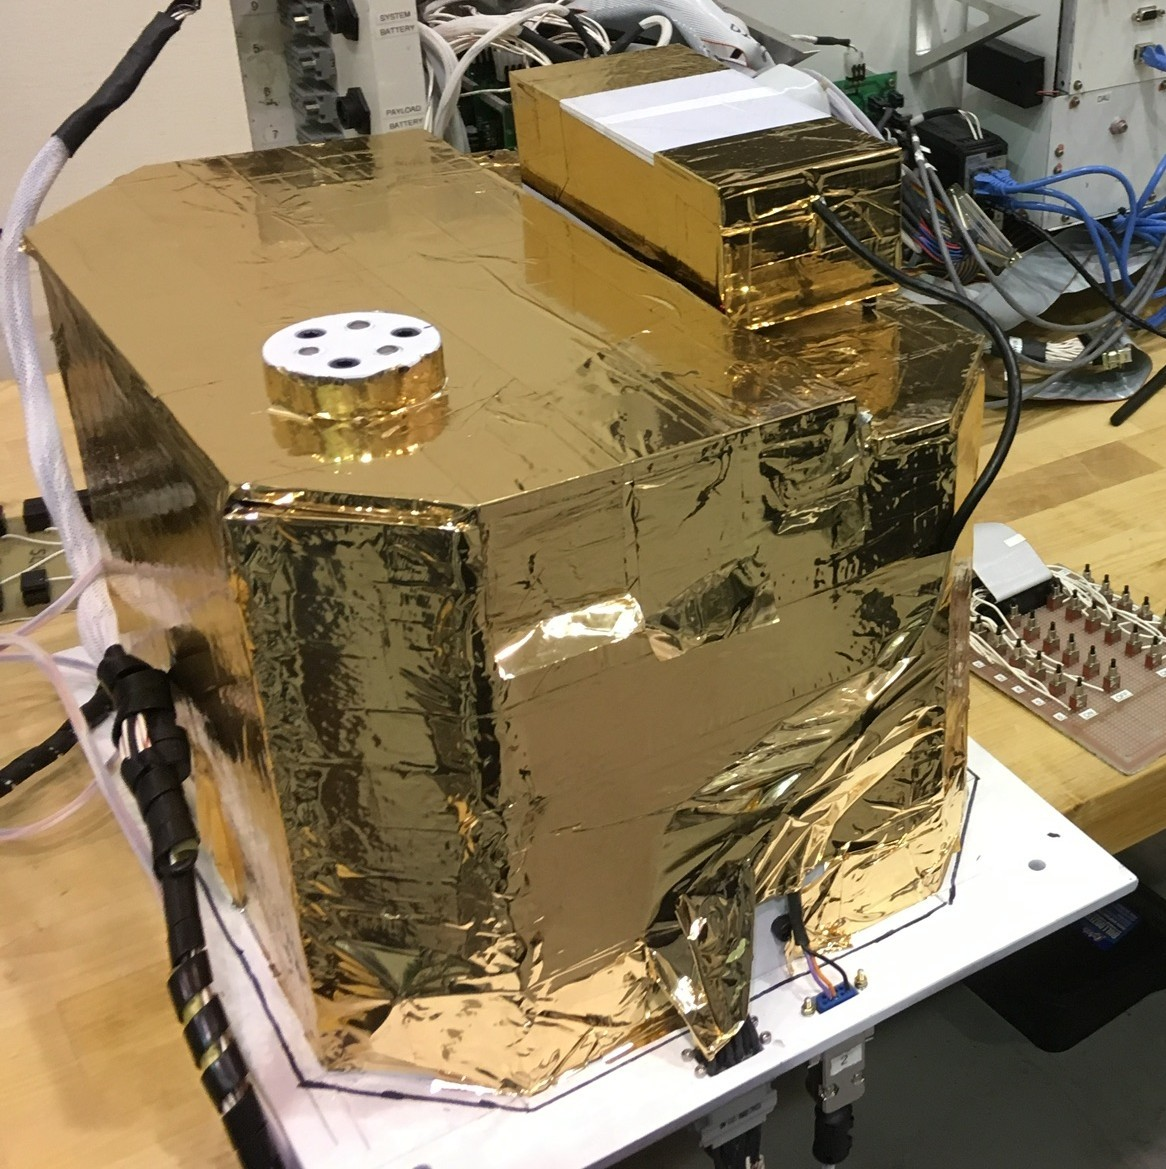
\includegraphics[width=\textwidth]{./Figures/sora.JPG}
      %\caption{SORA payload and main view of design.}
      \label{fig:payload} 
    \end{minipage}
    \hfill
    \begin{minipage}[c]{0.49\linewidth}
      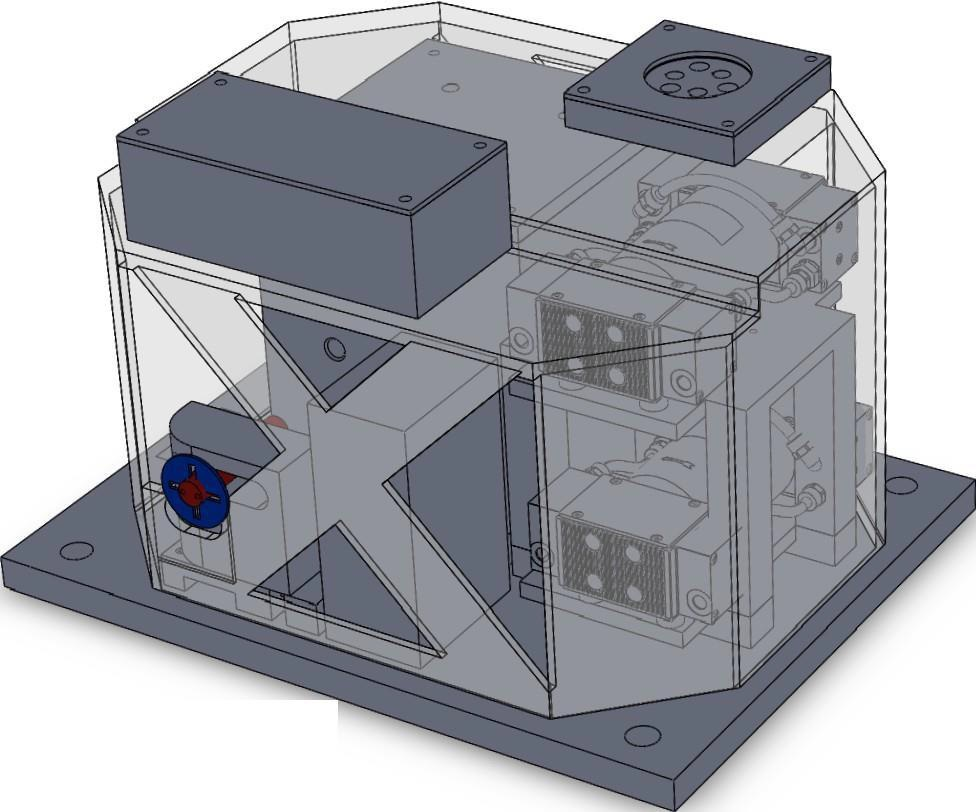
\includegraphics[width=\textwidth]{./Figures/payload_1.jpg}
      %\caption{Main view of the original payload design.}
      \label{fig:Payload_1}
    \end{minipage}
  \end{center}
        \caption{{\bf Left:} Picture of the completed SORA payload.  {\bf Right:} 3d rendering of the SORA payload.}
\end{figure}


The SORA payload was composed of two main systems controlled by RESU (Real-time Environmental Sensing Unit).  The first system is the astrobiology payload, composed of a vacuum pump, tubing, solenoid, and clean box with sample collection cells.  The second system is the radiation package.  It consists of a MiniPIX USB silicon chip-based particle detector and a series of three identical UV diodes.  RESU controls each system and in addition, monitors the surrounding environment through various temperature, pressure, and humidity sensors.  

In the following payload figures we show our final designs before flight.  There were two critical changes in the months before flight to remove one pump and cut the clean box in half before flight. This was necessary to stay within power, weight and space requirements for HASP.  The outer shell was made of Kydex sheets, which is composed of  acrylic and PVC material.  All other parts and housings were 3D printed out of ABS and PLA plastics.  The clean box was manufactured out of ultra-high molecular weight polyethylene (UHMWPE) since it can be autoclaved for astrobiology use.  

%too much white space below this paragraph, we need to fill it up or fix it somehow

%\newpage
%\begin{figure}[t!]
%\begin{center}
%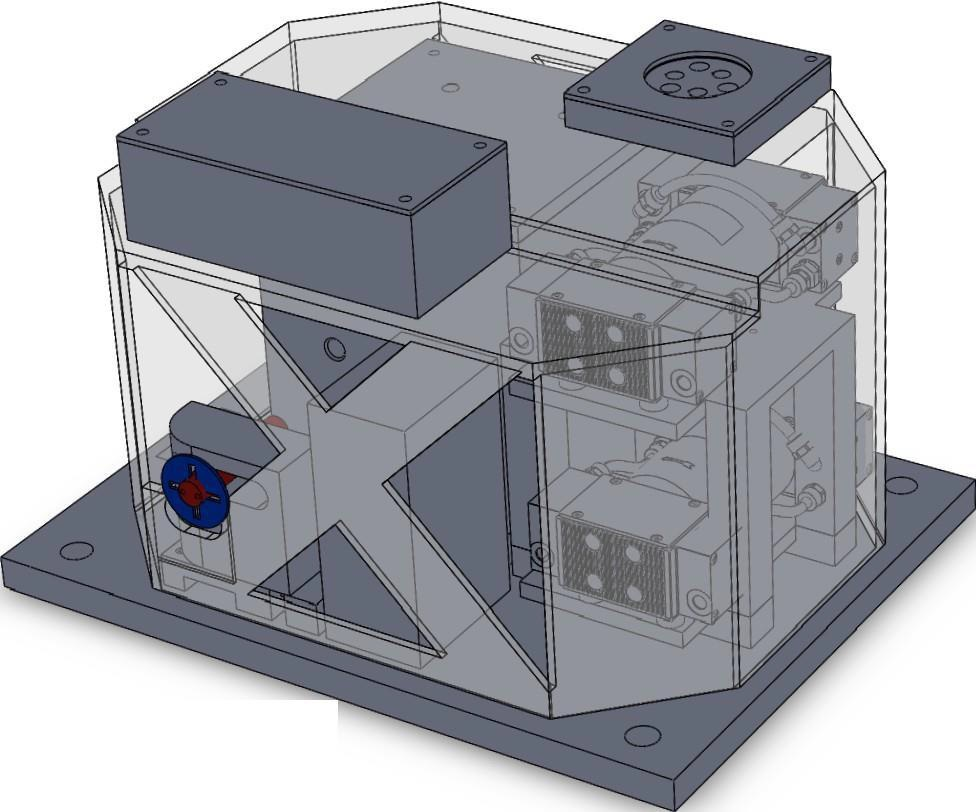
\includegraphics[width=0.5\textwidth]{./Figures/payload_1.jpg}
%\caption{Main view of the original payload design.}
%\label{fig:Payload_1}
%\end{center}
%\end{figure}

%\begin{figure}[!htb]
%\begin{center}
%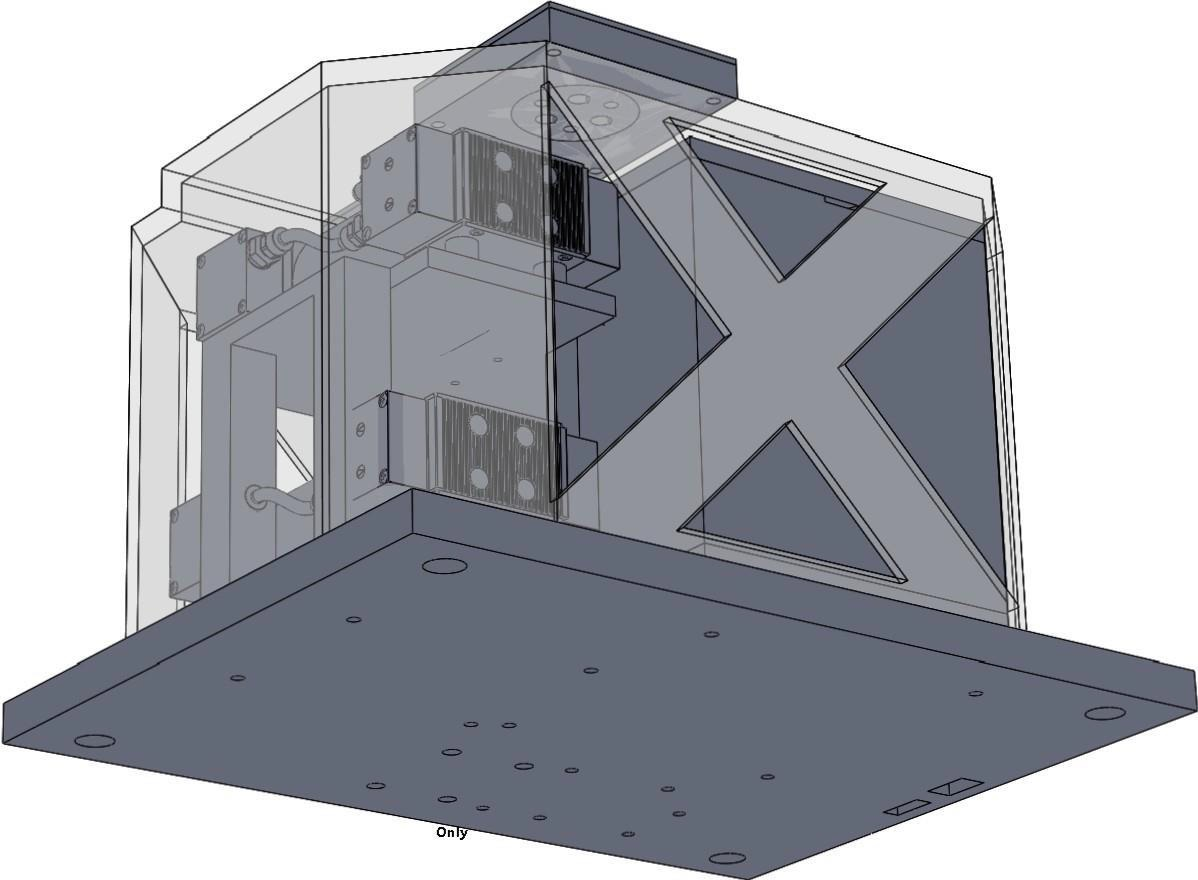
\includegraphics[width=0.5\textwidth]{./Figures/payload_2.jpg}
%\caption{An additional view of the payload design.}
%\label{fig:Payload_2} 
%\end{center}
%\end{figure}

%\begin{figure}[!htb]
%\begin{center}
%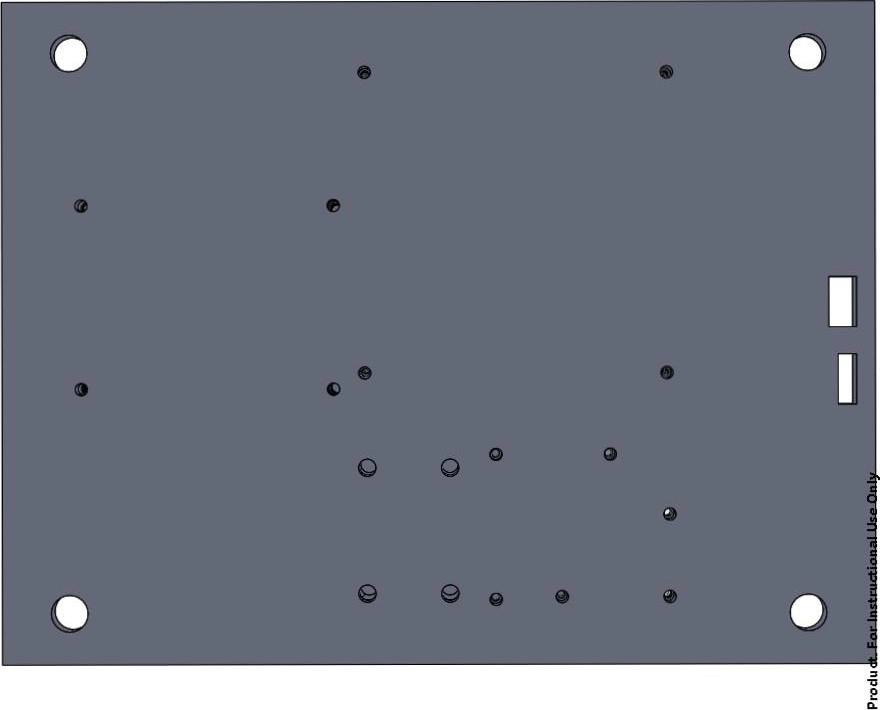
\includegraphics[width=0.5\textwidth]{./Figures/payload_3.jpg}
%\caption{Bottom view of the plate mount.}
%\label{fig:Payload_3} 
%\end{center}
%\end{figure}

%\begin{figure}[!htb]
%\begin{center}
%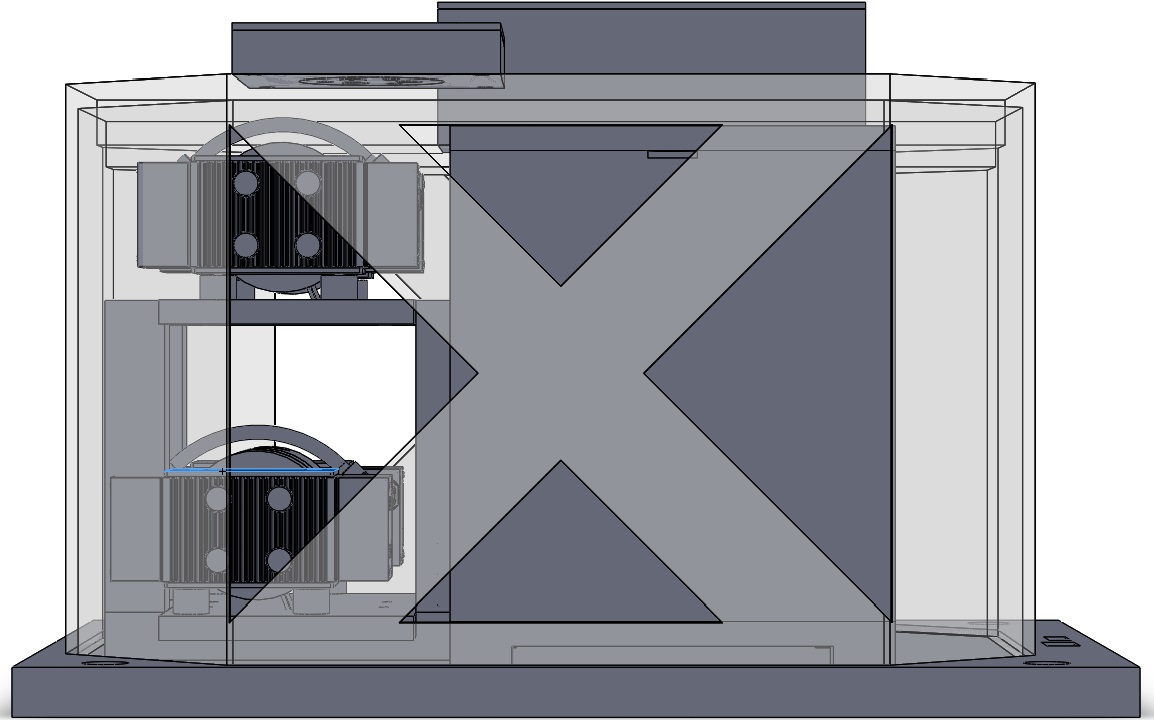
\includegraphics[width=0.5\textwidth]{./Figures/payload_4.jpg}
%\caption{Side view of payload design.}
%\label{fig:Payoad_4} 
%\end{center}
%\end{figure}
